\section[Floquetifying the $\qcode{4, 2, 2}$ code]{Floquetifying the $\mathbf{\qcode{4, 2, 2}}$ code}\label{sec:floquetifying_422}
% Optional argument used by table of contents - no mathbf needed.

Let's return to our old friend the $\qcode{4,2,2}$ code, which we first met in \Cref{ex:422_stabilizer_code}.
This is a static stabilizer code, so we can write it as a dynamic stabilizer code with a length-1 operation sequence $\OOO = (\{Z_1 Z_2 Z_3 Z_4, X_1 X_2 X_3 X_4\})$ (where again we're abusing notation and just writing the Pauli $P$ to be measured, rather than the full operation $M_P$).
%As a warm-up, we will show that this code can be reinterpreted as a 12-qubit Floquet code.
Recall that the notation $\qcode{n, k, d}$ means the code uses $n$ physical qubits to encode $k$ logical ones with an algebraic distance of $d$, and we defined algebraic distance for static and dynamic stabilizer codes (\Cref{subsec:distance,subsec:dynamic_distance}).
As a warm-up, we will prove the following:

\begin{theorem}\label{thm:4_2_2_double_hexagon_equivalence}
    The $\qcode{4, 2, 2}$ stabilizer code can be reinterpreted as a $\qcode{12, 2, 2}$ Floquet code with period 6, which we call the \textbf{double hexagon code}.
\end{theorem}

In \Cref{fig:4_2_2_rewritten}, we show three equivalent ZX-diagrams depicting seven timesteps of this code.
Here the grey squares, grey numbers, wire colours and wire styles (solid/dashed) have no meaning in the ZX-calculus;
they're just visual aids.
The grey squares denote timesteps of the $\qcode{4, 2, 2}$ code, and the grey numbers and coloured/styled lines will be explained shortly.
The leftmost diagram is the most natural one;
it shows measurements of $Z_1 Z_2 Z_3 Z_4$ and $X_1 X_2 X_3 X_4$ alternating at each timestep.
The second diagram is obtained from the first by unfusing every spider in the center of a grey square into two spiders,
and unfusing every spider in the corner of a grey square into three spiders.
The third is identical to the second in the ZX-calculus - all we've done is coloured and styled certain wires,
and labelled all one-legged spiders and black wires with an integer.
Now, in the leftmost diagram,
we interpret the four vertical lines as the world-lines of the four qubits of the code.
But we need not do this!
The ZX-diagram remains equivalent if we choose to interpret different wires as qubit world-lines.
This is exactly what the colours and styles in the rightmost diagram are for;
each colour-style pair denotes a different qubit world-line.
Since there are twelve world-lines, we're now viewing this as a system of twelve qubits, rather than four.
\begin{figure}[t]
    \centering
    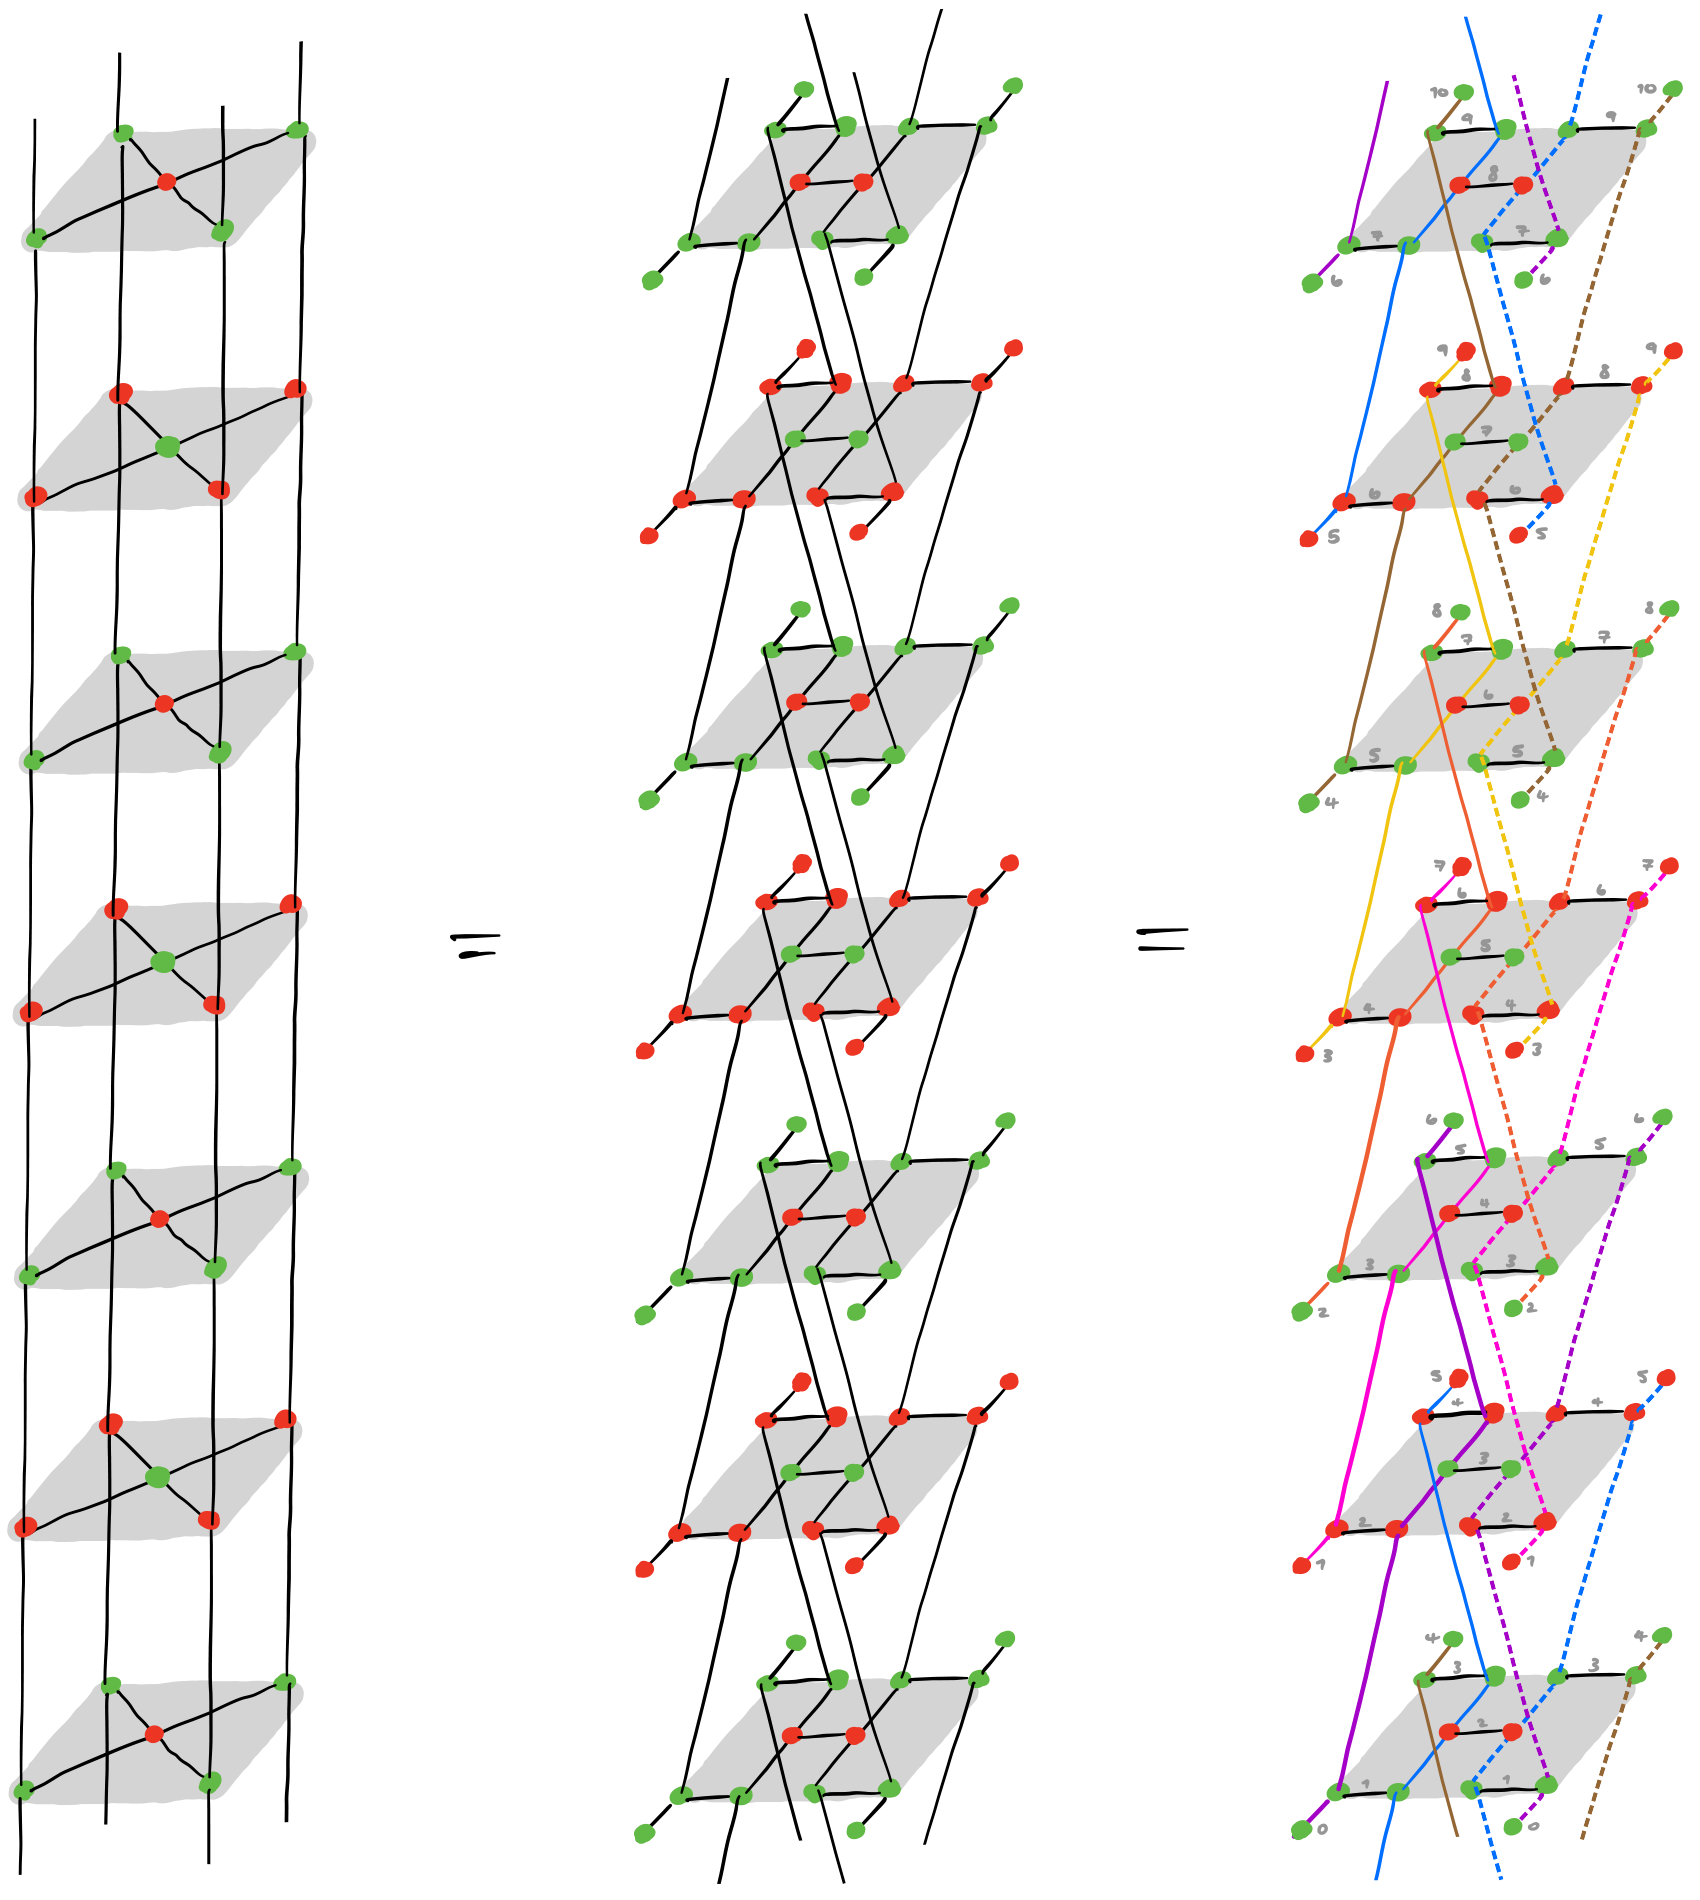
\includegraphics[width=340pt]{figures/qubits/floquetifying/422/zx_rewritten}
    \caption{Three equivalent ZX-diagrams for seven timesteps of the $\qcode{4, 2, 2}$ code.}
    \label{fig:4_2_2_rewritten}
\end{figure}

Let's make some observations about this rightmost diagram.
Firstly, if we follow the world-line of any particular qubit up the page,
the integer labels incident to it form an increasing sequence.
For example, starting from the bottom of the diagram and following the solid purple qubit upwards,
the integers incident to it form the sequence $[0, 1, \ldots, 6]$.
We can thus think of these integers as a new set of timesteps for this diagram.
Next, notice that we can interpret all the uncoloured black wires like
\ 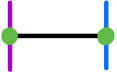
\includegraphics[height=1\baselineskip, valign=c]{figures/qubits/floquetifying/zx_calculus/ZZ}
\ and
\ 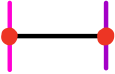
\includegraphics[height=1\baselineskip, valign=c]{figures/qubits/floquetifying/zx_calculus/XX}
\ as weight two $Z_u Z_v$ and $X_u X_v$ measurements (respectively) between qubits.
Furthermore, the qubit world-lines only have limited interactions with each other via these measurements.
Specifically, if we define sequences
$\mathbf{colours} = (
\mathbf{purple}, ~
\mathbf{pink}, ~
\mathbf{orange}, ~
\mathbf{yellow}, ~
\mathbf{brown}, ~
\mathbf{blue})$
and
$\mathbf{styles} = (
\mathbf{solid}, ~
\mathbf{dashed})$,
and let qubit $(i, j)$ denote the qubit with the $i$-th colour and $j$-th style,
where $i$ and $j$ are taken modulo 6 and 2 respectively,
then looking closely we see that qubit $(i, j)$ is only ever involved in
a measurement with the three qubits $(i+1, j), (i-1, j)$ and $(i, j+1)$.
So supposing we now wanted to lay out these qubits on a planar 2D chip,
a natural geometry would be a `double hexagon', as in the rightmost diagram of \Cref{fig:detector_4_2_2_double_hexagon}.

In fact, recalling the diagrammatic equation\
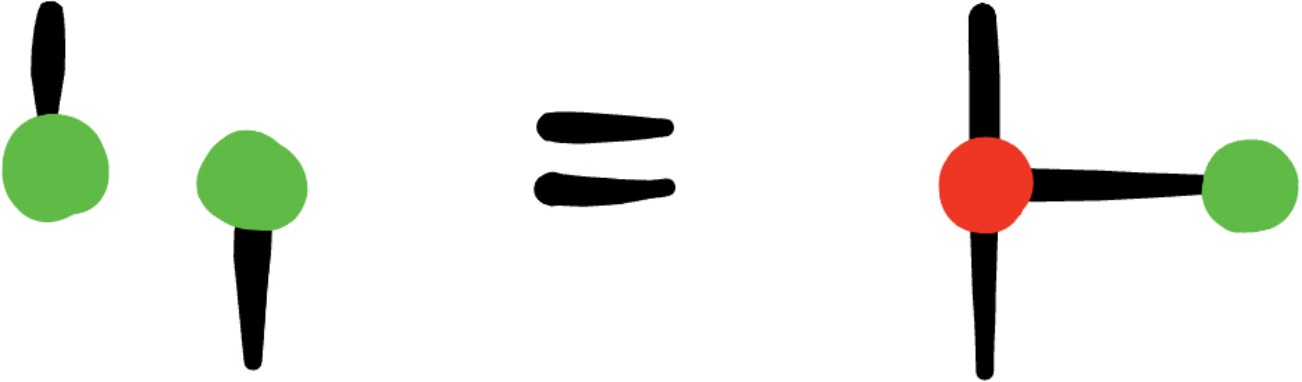
\includegraphics[height=1.1\baselineskip, valign=c]{figures/qubits/floquetifying/zx_calculus/single_qubit_measurement_splits}\ ,
which says that non-destructive single qubit Pauli measurements disconnect wires,
we can also interpret all one-legged spiders as one half of such a measurement.
This interpretation is valid,
in that the timestep at which the world-line of qubit $(i, j)$ `ends' at a one-legged spider
is the same as the timestep at which it `resumes' via another one-legged spider further up the page.
Finally, we can see that this pattern of colours and styles repeats itself every six timesteps.

From this analysis, we can now interpret the rightmost ZX-diagram as a dynamic stabilizer code;
we can write down the measurements that each qubit undergoes at each timestep,
and consequently we can define the operation sequence described by this diagram.
We get $\OOO = (\OOO_0, \ldots, \OOO_5)$, where:
\begin{equation}\label{eq:floquetified_4_2_2_measurement_schedule}
    \begin{aligned}
        \OOO_t &= \left\{
        \begin{array}{l}
             X_{(t, 0)}, \\
             X_{(t, 1)}, \\
             X_{(t+1, 0)}X_{(t+2, 0)}, \\
             X_{(t+1, 1)}X_{(t+2, 1)}, \\
             X_{(t+3, 0)}X_{(t+3, 1)}, \\
             X_{(t+4, 0)}X_{(t+5, 0)}, \\
             X_{(t+4, 1)}X_{(t+5, 1)}
        \end{array}
        \right\}
        \text{~~if $t$ even,} \\[10pt]
        \OOO_t &= \left\{
        \begin{array}{l}
             Z_{(t, 0)}, \\
             Z_{(t, 1)}, \\
             Z_{(t+1, 0)}Z_{(t+2, 0)}, \\
             Z_{(t+1, 1)}Z_{(t+2, 1)}, \\
             Z_{(t+3, 0)}Z_{(t+3, 1)}, \\
             Z_{(t+4, 0)}Z_{(t+5, 0)}, \\
             Z_{(t+4, 1)}Z_{(t+5, 1)}
        \end{array}
        \right\}
        \text{~~if $t$ odd.}
    \end{aligned}
\end{equation}
One can then calculate the sequence of stabilizer groups $\SSS_t$ and logical Pauli groups $\LLL_t$.
It turns out $\SSS_t$ is established whenever $t \geq T = 3$,
and can be minimally generated by the seven elements of $\OOO_t$,
plus three weight-six Paulis $S_{t-1}, S_{t-2}$ and $S_{t-3}$, where:
\begin{equation}\label{eq:floquetified_4_2_2_s_t}
S_t = \begin{cases}
          X_{(t, 0)}X_{(t, 1)}X_{(t-1, 0)}X_{(t-1, 1)}X_{(t-2, 0)}X_{(t-2, 1)} &\text{ if $t$ even} \\
          Z_{(t, 0)}Z_{(t, 1)}Z_{(t-1, 0)}Z_{(t-1, 1)}Z_{(t-2, 0)}Z_{(t-2, 1)} &\text{ if $t$ odd} \\
\end{cases}
\end{equation}

Since we have 10 independent generators on 12 qubits, we can conclude that $\lpg{t} \cong \PPP_2$ for all $t \geq 3$.
This then proves most of \Cref{thm:4_2_2_double_hexagon_equivalence};
namely that the double hexagon code encodes 2 logical qubits and has period 6.
It remains to show the algebraic distance is still 2.

For the $\qcode{4, 2, 2}$, we can essentially do this by hand.
First, we can use the Pauli webs to find representatives of logical operators in the new code -- these are examples of logical errors under the phenomenological noise model, so give an upper bound on the algebraic distance.
In \Cref{fig:double_hexagon_x_1} we show the logical web corresponding to logical operator $\ol{\XXX}_1$ in the new code.
In particular, in the rightmost diagram of this figure, we show seven timesteps $t \in \{0, \ldots, 6\}$ of the period-six double hexagon code.
So looking at the output wires of this diagram tells us a representative of the logical $\ol{\XXX}_1$ at timestep $t=6$; we see the corresponding logical operator at this timestep is $X_{(0, 0)} X_{(0, 1)} X_{(5, 0)} X_{(5, 1)}$.
To see the corresponding logical operator at a different timestep $t$,
we can just truncate the diagram after timestep $t$ and again look at the highlighted output edges.
This is shown for timesteps $t \in \{0, 1, 2\}$ in \Cref{fig:double_hexagon_x_1_truncations} below;
the corresponding operators are
$X_{(0, 0)} X_{(0, 1)} X_{(5, 0)} X_{(5, 1)}$ after timesteps $t=0$ and $t=1$, and
$X_{(2, 0)} X_{(2, 1)} X_{(1, 0)} X_{(1, 1)}$ after timestep $t=2$.
In fact, truncating the rightmost diagram of \Cref{fig:double_hexagon_x_1} after \textit{any} timestep $t$
gives a logical web whose corresponding $\ol{\XXX}_1$ representative has weight four.

Next, one can find stabilizers at a given timestep $t$ with which to multiply these logical operators,
in order to reduce their weight to two.
One can do this algebraically,
making use of the fact that we already worked out the stabilizer groups $\SSS_t$ of the double hexagon code for all $t$.
Alternatively, one can do this graphically,
using the fact that Pauli webs on the same diagram form a group
and can thus be multiplied together.
In \Cref{fig:double_hexagon_x_1_truncations_multiplied} below,
we thus multiply the weight-four logical webs by appropriate stabilizing webs
to get weight-two logical webs.

This gives us an upper bound of two for the algebraic distance.
Since this code is fairly small, we can then check by hand that for no logical error under the phenomenological noise model has weight one.
Hence, the code has algebraic distance two, as promised.

\begin{figure}[p]
    \centering
    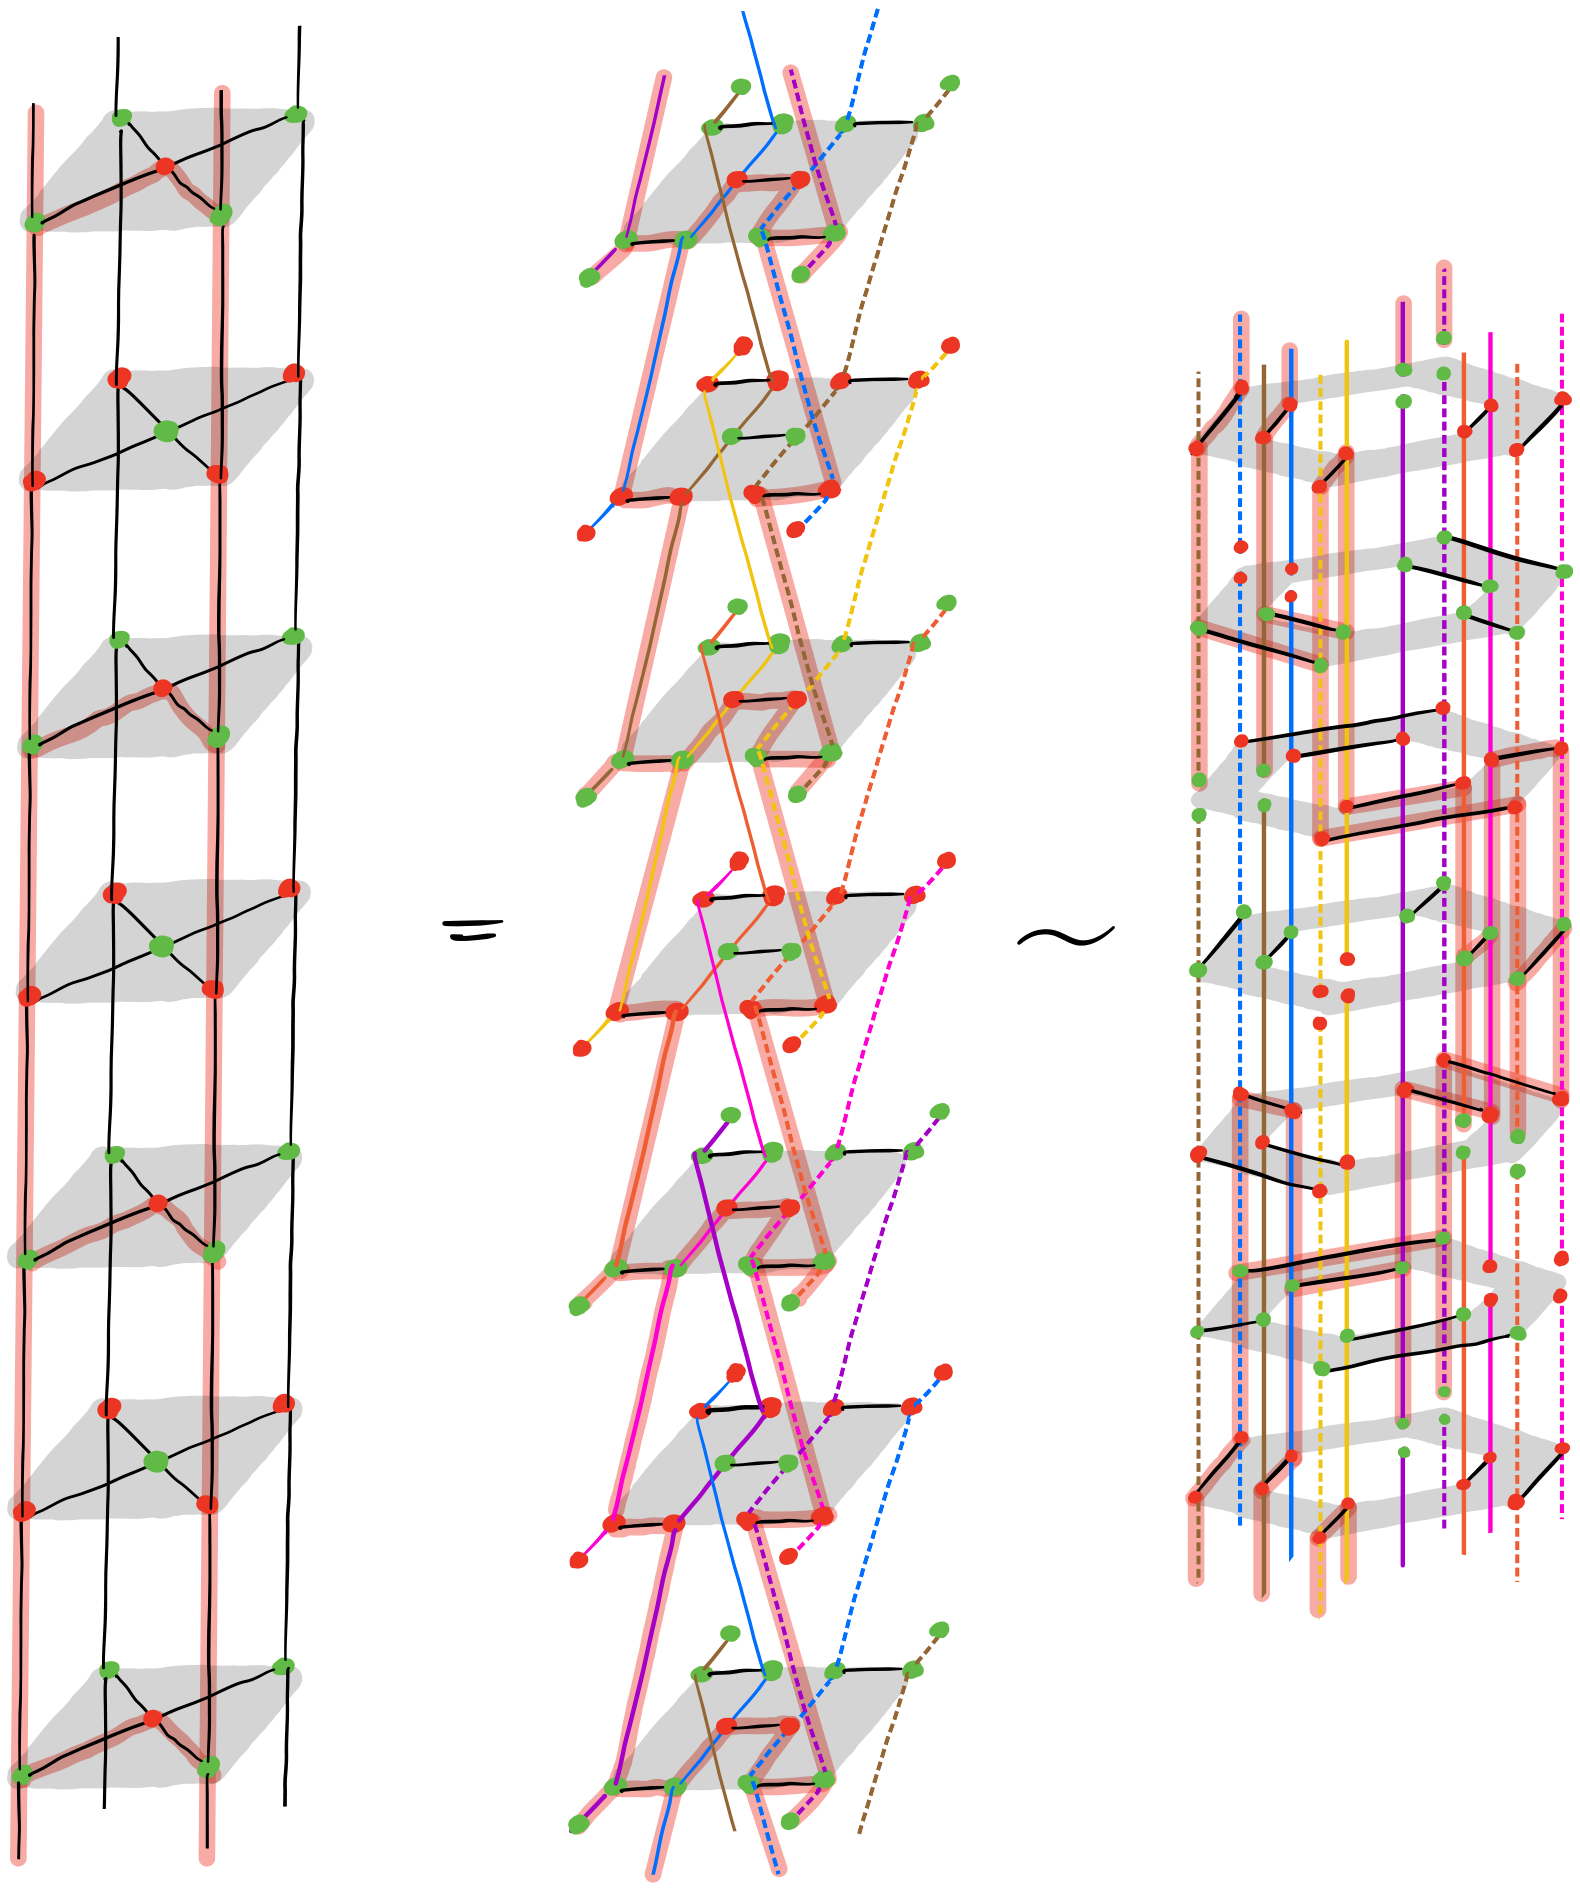
\includegraphics[width=\linewidth]{figures/qubits/floquetifying/422/floquetified/x_1}
    \caption{%
        A logical web corresponding to a representative of the logical $\ol{\XXX}_1$ in
        the $\qcode{4, 2, 2}$ code (left and middle)
        and in its Floquetification, the double hexagon code (right).}
    \label{fig:double_hexagon_x_1}
\end{figure}

%\begin{figure}[p]
%    \centering
%    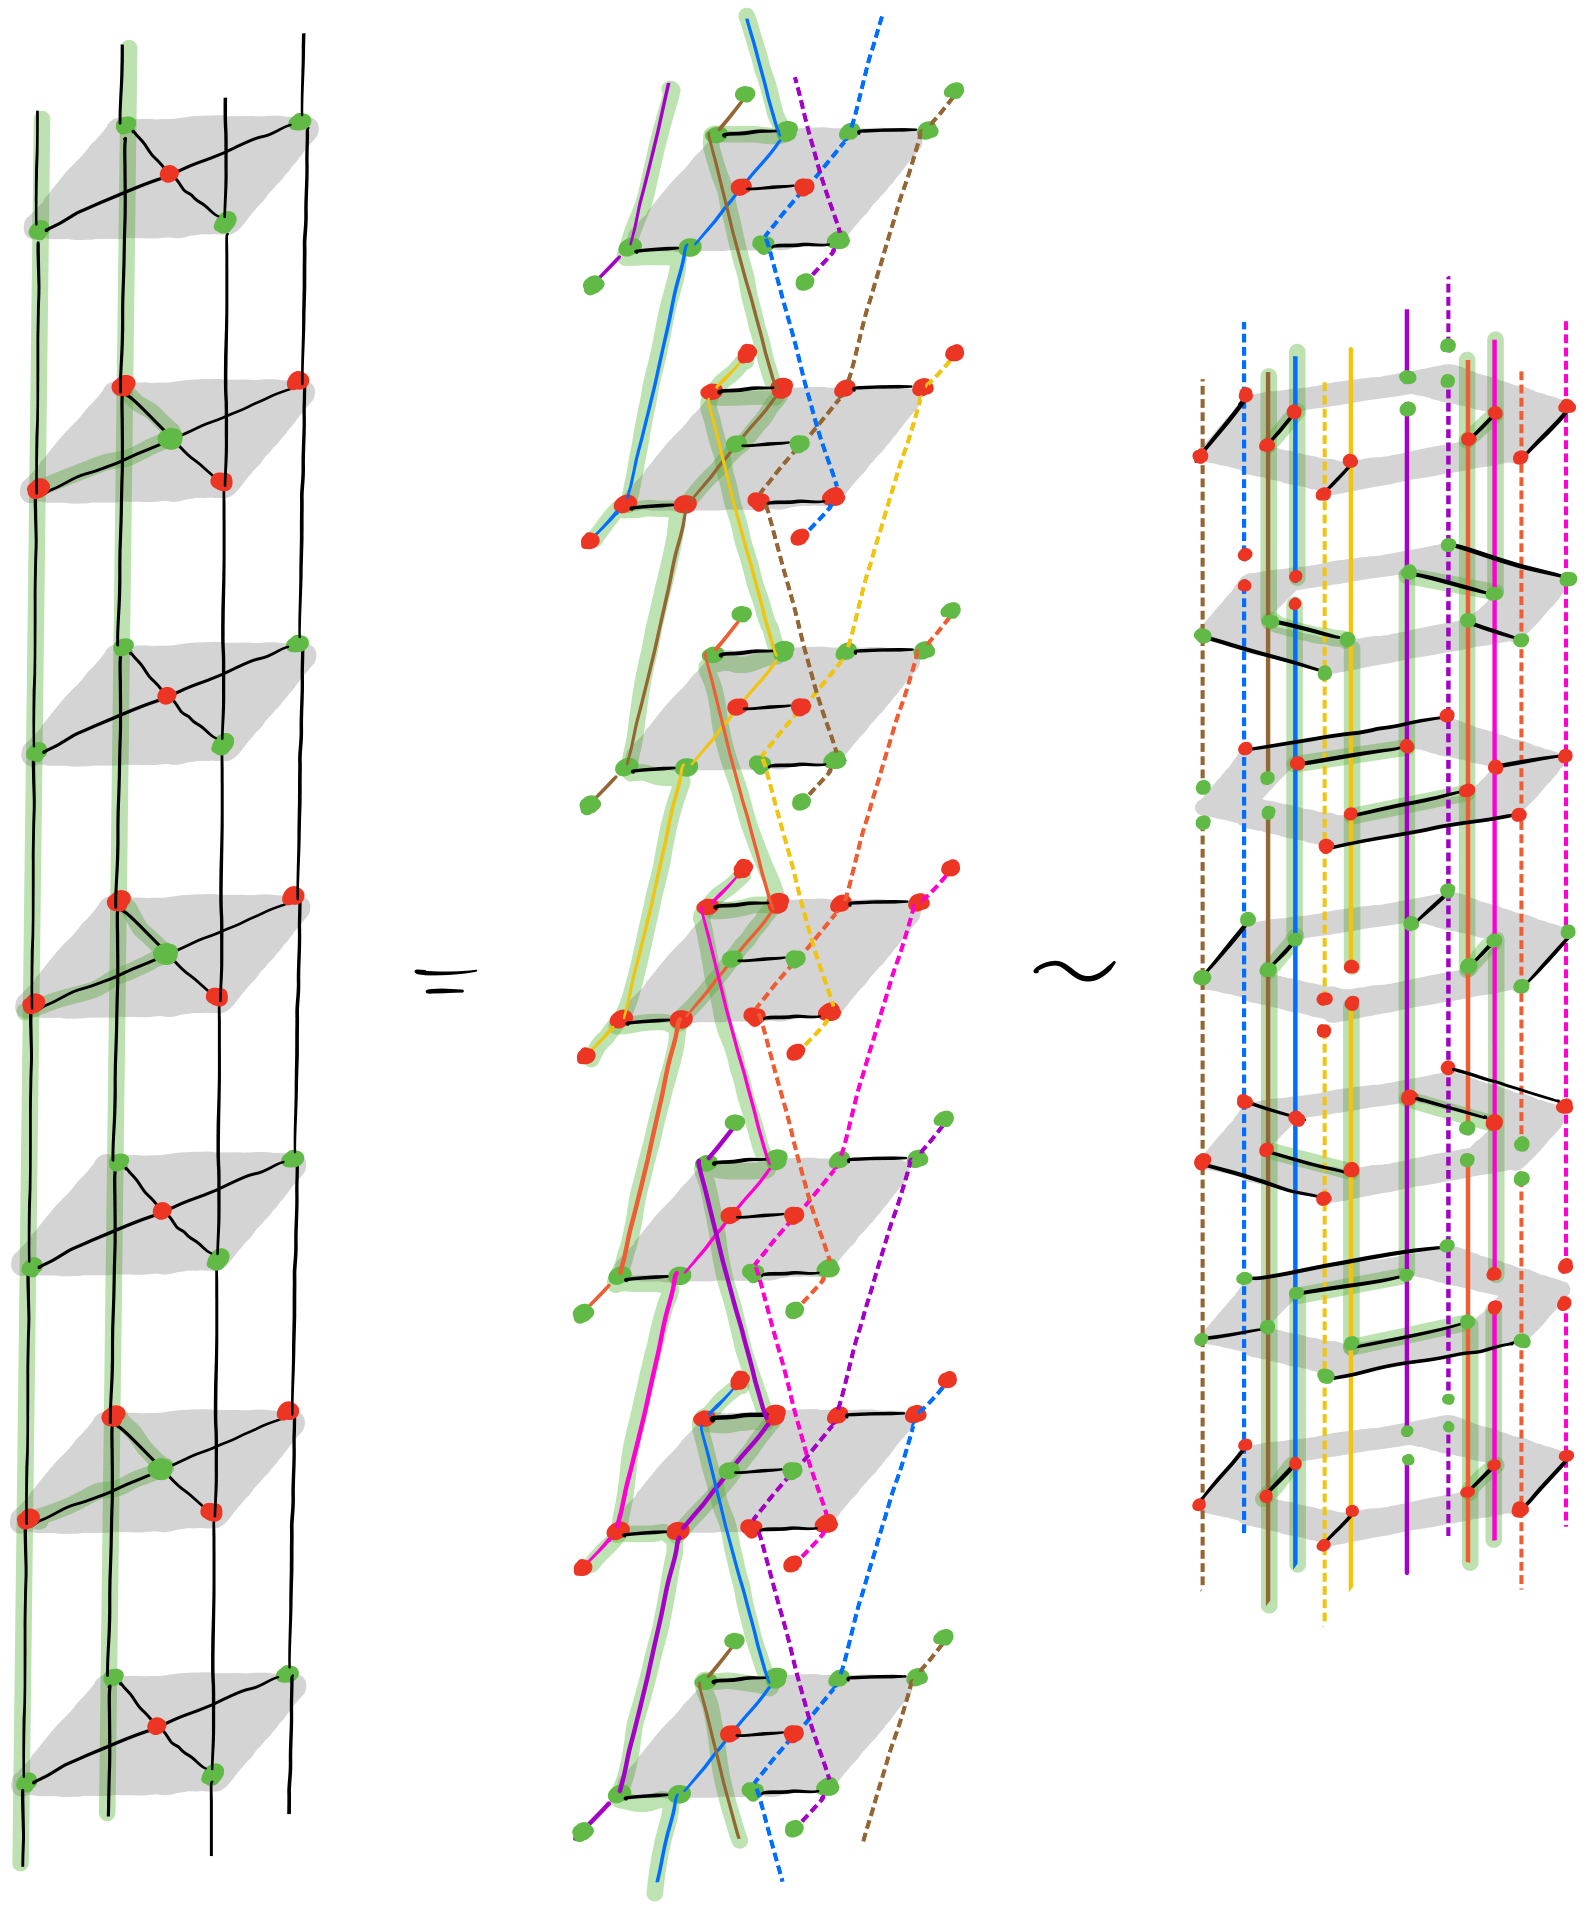
\includegraphics[width=\linewidth]{figures/qubits/floquetifying/422/floquetified/z_1}
%    \caption{%
%        A logical web corresponding to a representative of the logical $\ol{\ZZZ}_1$ in
%        the $\qcode{4, 2, 2}$ code (left and middle)
%        and in its Floquetification, the double hexagon code (right).}
%    \label{fig:double_hexagon_z_1}
%\end{figure}

\begin{figure}[p]
    \centering
    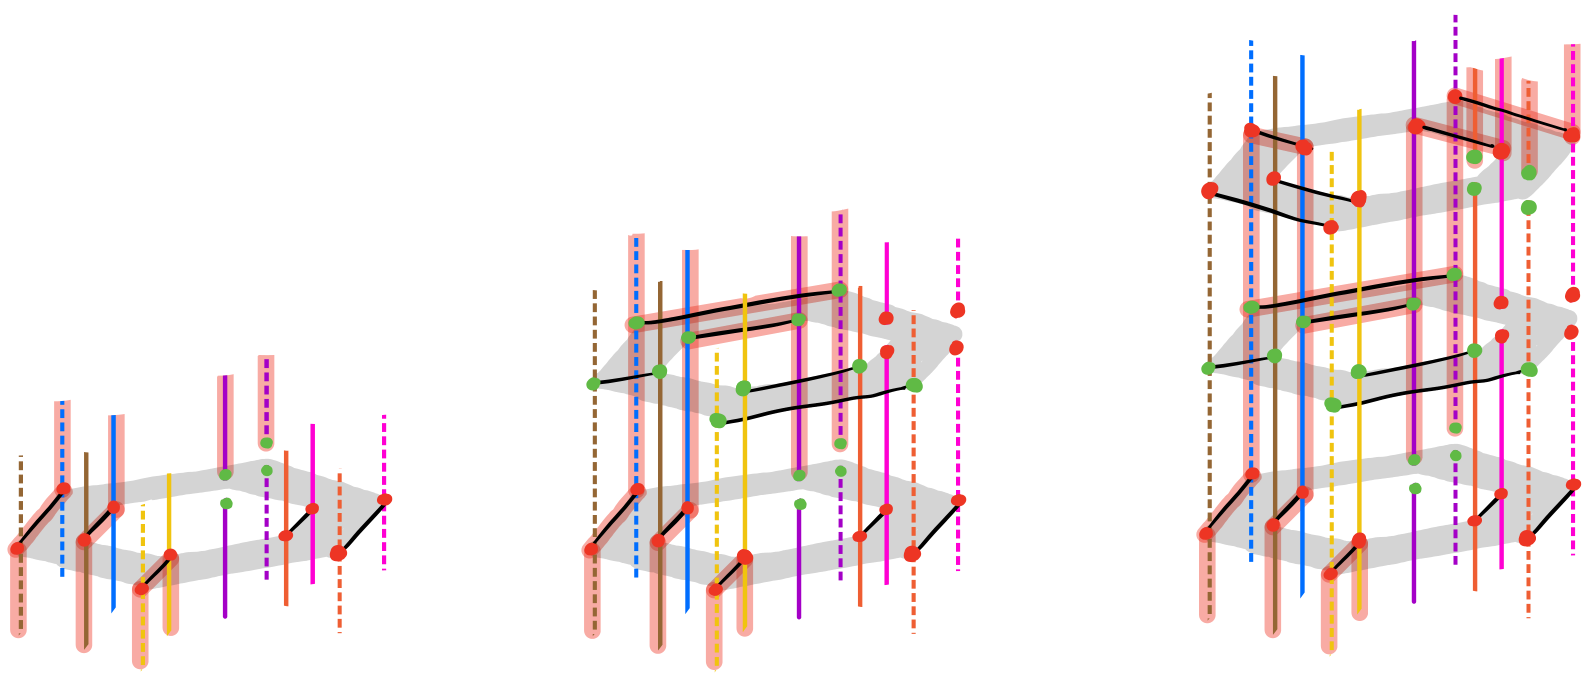
\includegraphics[width=\linewidth]{figures/qubits/floquetifying/422/floquetified/x_1_truncations}
    \caption{%
        The double hexagon code after timesteps $t=0$, $t=1$ and $t=2$ respectively,
        annotated with a logical web corresponding to a representative of the logical $\ol{\XXX}_1$.}
    \label{fig:double_hexagon_x_1_truncations}
\end{figure}

\begin{figure}[p]
    \centering
    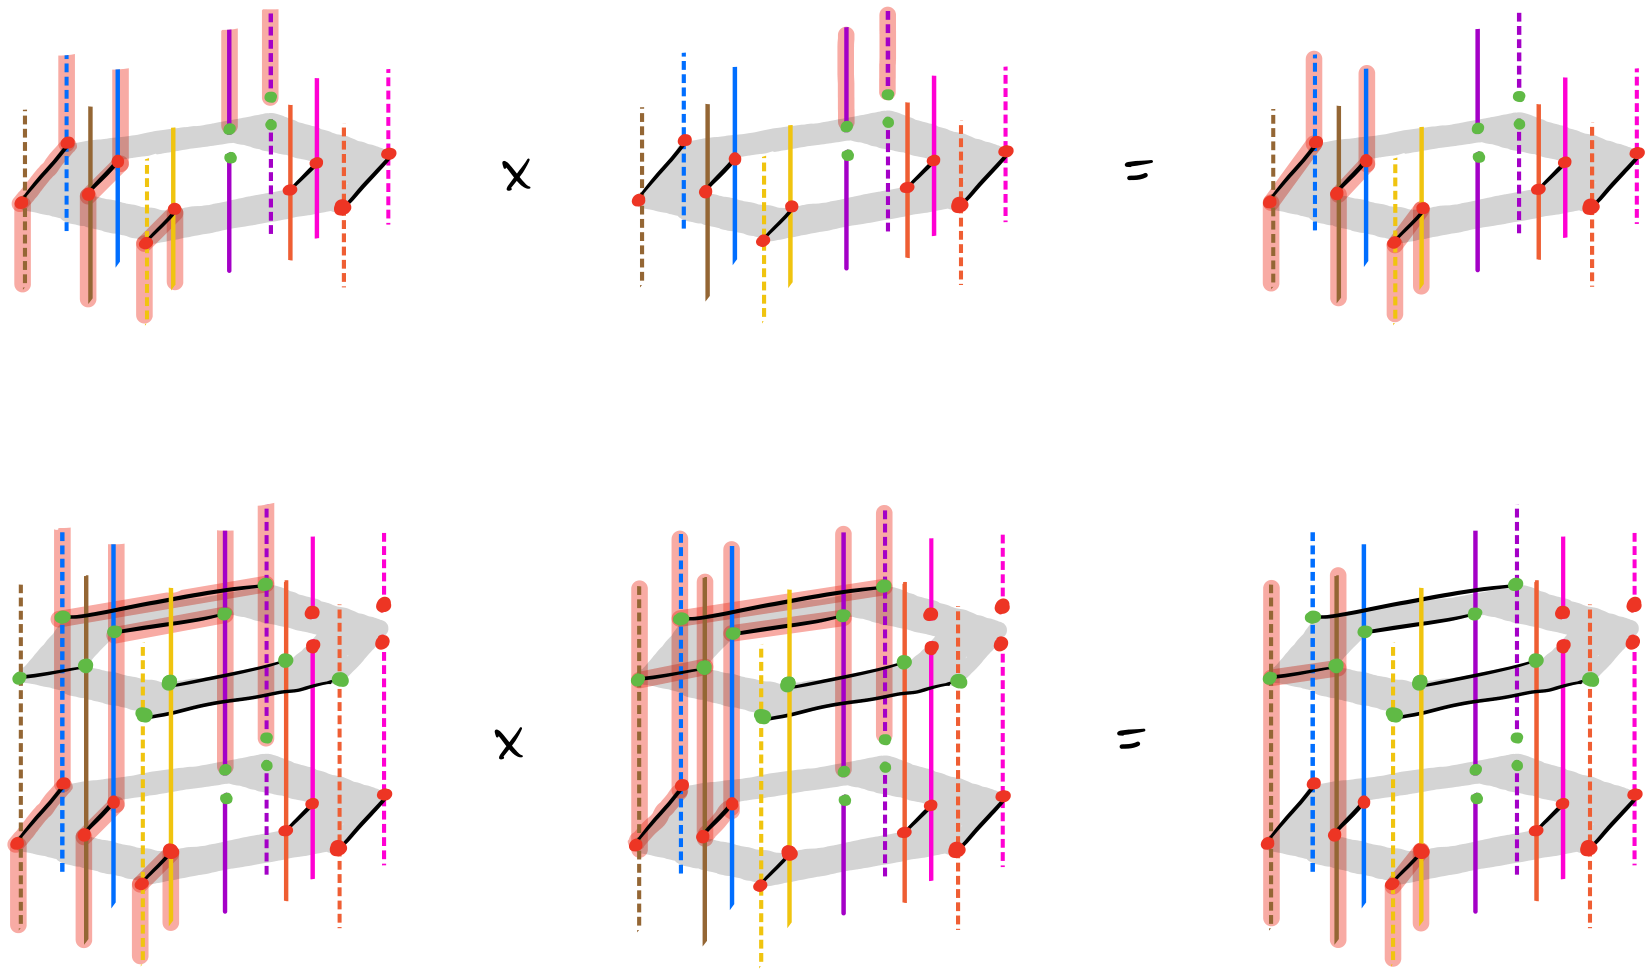
\includegraphics[width=\linewidth]{figures/qubits/floquetifying/422/floquetified/x_1_truncations_multiplied_0_1}
    \caption{%
    %        For timesteps $t=0$, $t=1$ and $t=2$ respectively,
        For timesteps $t=0$ and $t=1$ respectively,
        we multiply the weight-four logical webs of \Cref{fig:double_hexagon_x_1_truncations}
        by appropriate stabilizing regions, which gives us weight-two logical webs.
        This corresponds exactly to composition of the corresponding Pauli operators -
        for example, the topmost graphical equation corresponds to the algebraic equation
        $X_{(0, 0)} X_{(0, 1)} X_{(5, 0)} X_{(5, 1)} \after X_{(0, 0)} X_{(0, 1)} = X_{(5, 0)} X_{(5, 1)}$.}
    \label{fig:double_hexagon_x_1_truncations_multiplied}
\end{figure}

%To see the corresponding logical operator at a different timestep $t$,
%we can just truncate the diagram after timestep $t$ and again look at the highlighted output edges.
%This is shown for timesteps $t \in \{0, 1, 2\}$ in \Cref{fig:double_hexagon_x_1_truncations} below;
%the corresponding operators are
%$X_{(0, 0)} X_{(0, 1)} X_{(5, 0)} X_{(5, 1)}$ after timesteps $t=0$ and $t=1$, and
%$X_{(2, 0)} X_{(2, 1)} X_{(1, 0)} X_{(1, 1)}$ after timestep $t=2$.
%In fact, truncating the rightmost diagram of \Cref{fig:double_hexagon_x_1} after \textit{any} timestep $t$
%gives a logical web whose corresponding $\ol{\XXX}_1$ representative has weight four.
%The same is true for all possible truncations of the $\ol{\ZZZ}_1$ logical web in \Cref{fig:double_hexagon_z_1},
%and would also be true if we repeated this process for the other logical operator cosets $\ol{\XXX}_2$ and $\ol{\ZZZ}_2$.
%That is, truncating after timestep $t$ would always give us a logical web whose corresponding operator had weight four.
%It would be tempting to conclude, therefore, that the double hexagon code has distance four,
%and that Floquetifying the $\qcode{4, 2, 2}$ code has increased its distance.
%But this would be wrong!
%
%The reason is that while this process gives us logical operators in the Floquetification,
%it doesn't necessarily give us minimum-weight ones,
%even though we started with minimum-weight logical webs of the $\qcode{4, 2, 2}$ code in
%the leftmost diagrams of \Cref{fig:double_hexagon_x_1,fig:double_hexagon_z_1}.
%Indeed, one can find stabilizers at a given timestep $t$ with which to multiply these logical operators,
%in order to reduce their weight to two.
%One can do this algebraically,
%making use of the fact that we already worked out the stabilizer groups $\SSS_t$ of the double hexagon code for all $t$.
%Alternatively, one can do this graphically,
%using the fact that Pauli webs on the same diagram form a group
%and can thus be multiplied together.
%In \Cref{fig:double_hexagon_x_1_truncations_multiplied} below,
%we thus multiply the weight-four logical webs by appropriate stabilizing webs
%to get weight-two logical webs.

%Since this code is fairly small, one can use these ideas to check by hand that for all $t$,
%no logical operator at time $t$ has weight one.
%Hence, since representatives of weight two exist for the logical operator coset $\ol{\XXX}_1$,
%the code has distance two, as promised.
%It is interesting, however, that for the logical operator coset $\ol{\ZZZ}_1$,
%the weight of the smallest representative is four at all even timesteps,
%and three at all odd timesteps.
%The story is analogous on the other logical qubit;
%for $\ol{z_2}$ we can always find a weight-two representative for all timesteps $t$,
%but for $\ol{x_2}$ the weight of the smallest representatives alternates
%between three and four at odd and even timesteps respectively.
%This is in contrast to the $\qcode{4, 2, 2}$ code,
%which has a weight-two representative for all logicals at all timesteps.
%So Floquetifying this code seems to have increased the average-case code distance across all timesteps.
%However, as touched on in \Cref{sec:isg_code_remarks},
%we suspect that this is just a result of fact that our definition of an ISG code's distance is too rigid.

%\begin{figure}[h]
%    \centering
%    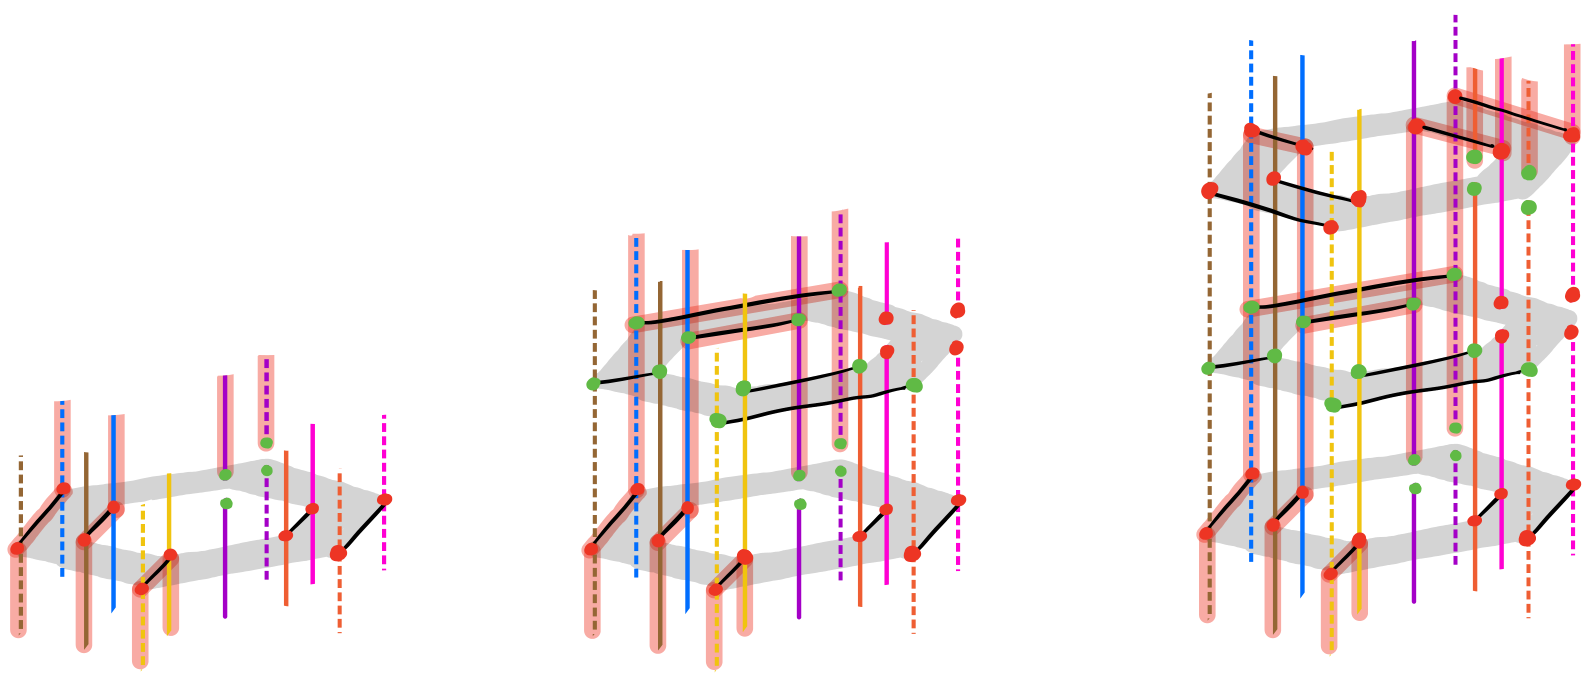
\includegraphics[width=450pt, valign=c]{figures/qubits/floquetifying/422/floquetified/x_1_truncations}
%    \caption{%
%        The double hexagon code after timesteps $t=0$, $t=1$ and $t=2$ respectively,
%        annotated with a logical web corresponding to a representative of the logical $\ol{\XXX}_1$.}
%    \label{fig:double_hexagon_x_1_truncations}
%\end{figure}

%In addition to being able to work with detectors, stabilizers and logical operators algebraically, as above,
%the mapping of these objects from the $\qcode{4, 2, 2}$ code to the double hexagon code
%can be seen graphically via Pauli webs.
In the proof above, we took a logical web on the $\qcode{4, 2, 2}$ code and looked at the corresponding web in the Floquetified diagram.
We can do this for any Pauli web we like.
For example, in \Cref{fig:detector_4_2_2_double_hexagon} we show a detecting region in the $\qcode{4, 2, 2}$ code
and its image in the double hexagon code.
From the rightmost diagram of this figure,
and recalling the rules for mapping a detecting region to a detector from \Cref{subsec:detecting_webs_detect_errors},
one can see that the corresponding detector in the double hexagon code consists of eight measurements.
Specifically, in the bottom layer, we include two $Z \otimes Z$ measurements between blue and purple qubits,
and two single qubit $Z$ measurements on pink qubits.
In the top layer, we include two $Z \otimes Z$ measurements between purple and pink qubits,
and two single qubit $Z$ measurements on blue qubits.
Since every detecting region in the $\qcode{4, 2, 2}$ code is equivalent to the one on the left of this figure
(up to a space-time translation and exchanging the roles of $Z$ and $X$),
every detecting region in the double hexagon code is equivalent to the one on the right
(again up to a space-time translation and $Z \leftrightarrow X$ interchange).

\begin{figure}[btp]
    \centering
    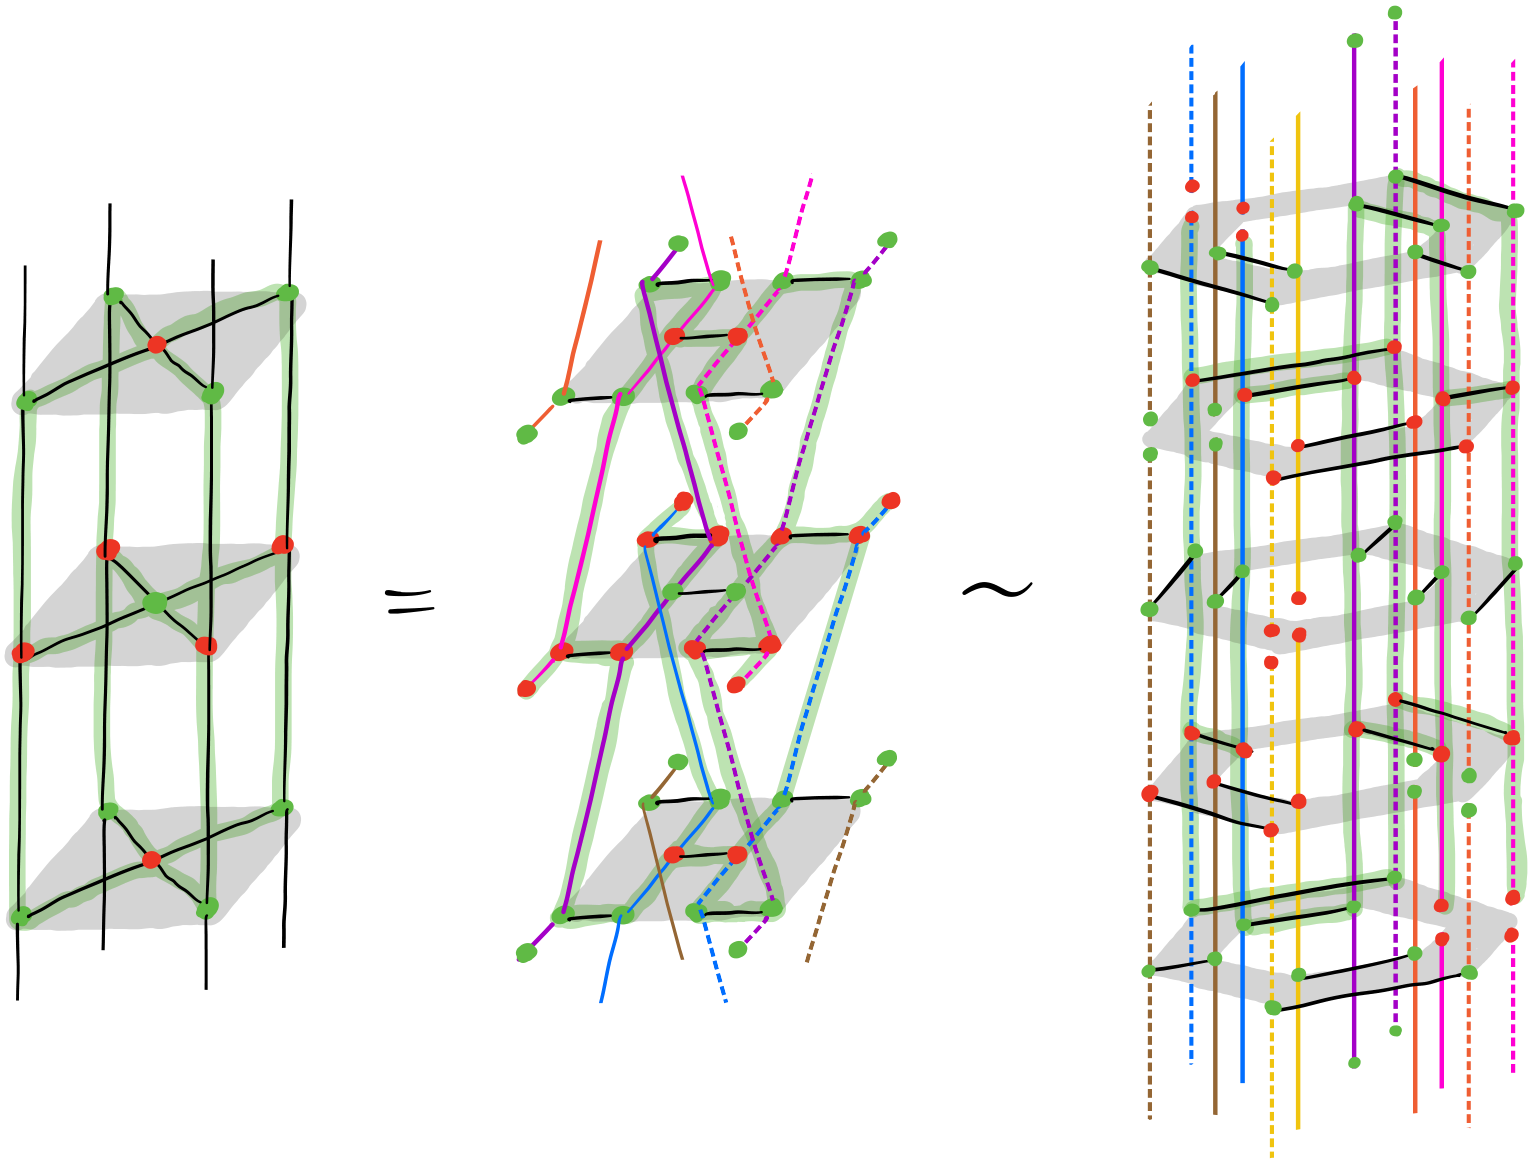
\includegraphics[width=330pt]{figures/qubits/floquetifying/422/floquetified/detector}
    \caption{
        A detecting region in the $\qcode{4, 2, 2}$ code and its image in the double hexagon code.
        We use the ($\sim$) symbol between the second and third diagrams rather than an equals sign because,
        although the two codes can be viewed as having equivalent ZX-diagrams,
        these two particular subdiagrams are not equivalent -
        the rightmost one has more input and output wires, for example.}
    \label{fig:detector_4_2_2_double_hexagon}
\end{figure}

So, summing up, we've taken a $\qcode{4, 2, 2}$ static stabilizer code and turned it into a $\qcode{12, 2, 2}$ dynamic stabilizer code, in which each detector now consists of eight measurements rather than two.
On paper, these are all changes for the worse!
The trade-off, as discussed in the introduction, is that now every measurement is weight-two or weight-one, rather than weight-four, so will be less noisy.

On a higher-level, one can view this Floquetification as a reinterpretation of the time direction
in a ZX-diagram.
Below, we use two blue prisms (square and hexagonal) as abstractions of ZX-diagrams for the $\qcode{4, 2, 2}$ code and double hexagon code respectively.
In grey we show how a timeslice in the double hexagon code corresponds to an angled slice of the $\qcode{4, 2, 2}$ code.
We will return to this perspective shortly.
\begin{equation}\label{eq:timeslice_4_2_2_double_hexagon}
\begin{aligned}
    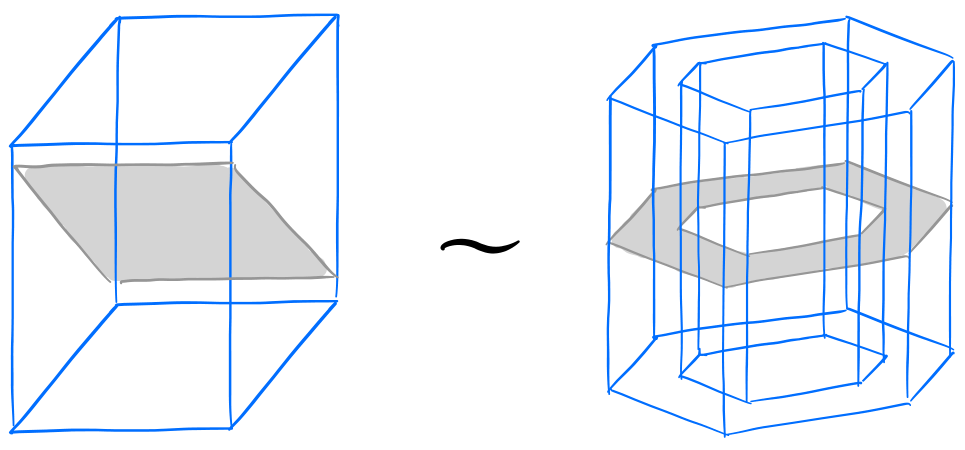
\includegraphics[width=230pt]{figures/qubits/floquetifying/422/floquetified/abstract_timeslice}
\end{aligned}
\end{equation}
